\chapter{Strain B-scan Images}\label{images}

This appendix shows the 2D B-scan images for the six different processing techniques at different fit and lateral resolutions. It is important to analyse the image as a whole, rather than just looking at sensitivity and image resolution, because artefacts may manifest in areas outside of those used to calculate these parameters. Also, these images provide a more intuitive understanding of the affect of changing the resolution parameters.

\begin{figure}[h]
	\centering
    \begin{subfigure}{0.49\textwidth}
    	\centering
        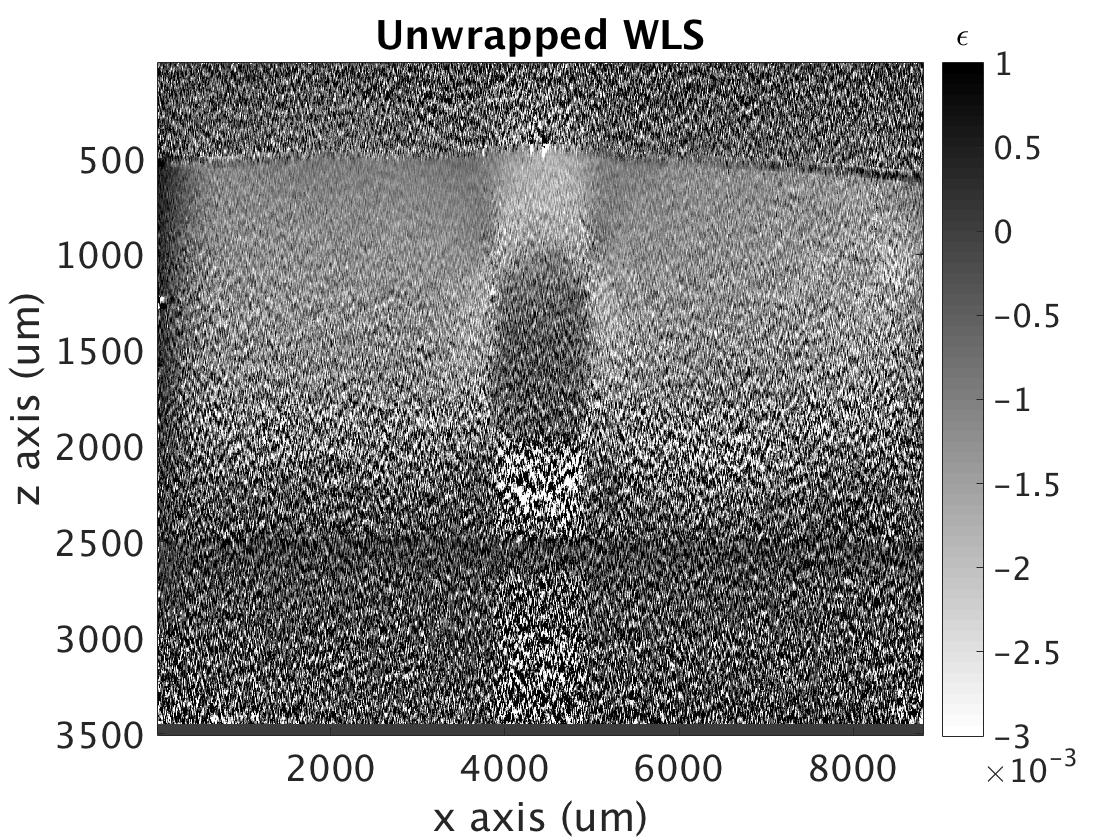
\includegraphics[width=\textwidth]{appendix_figs/wls_fr40_lr0.png}
    \end{subfigure}
    \begin{subfigure}{0.49\textwidth}
    	\centering
        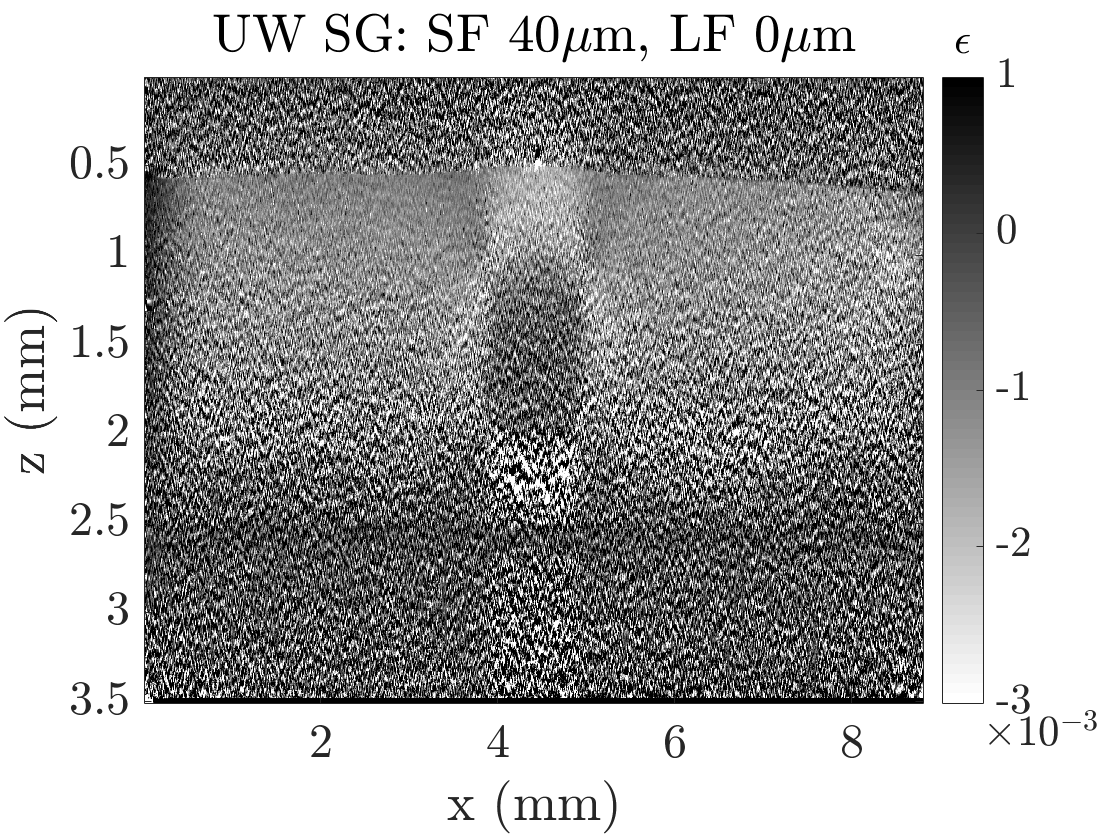
\includegraphics[width=\textwidth]{appendix_figs/uwsg_fr40_lr0.png}
    \end{subfigure}
    \\
    \begin{subfigure}{0.49\textwidth}
    	\centering
        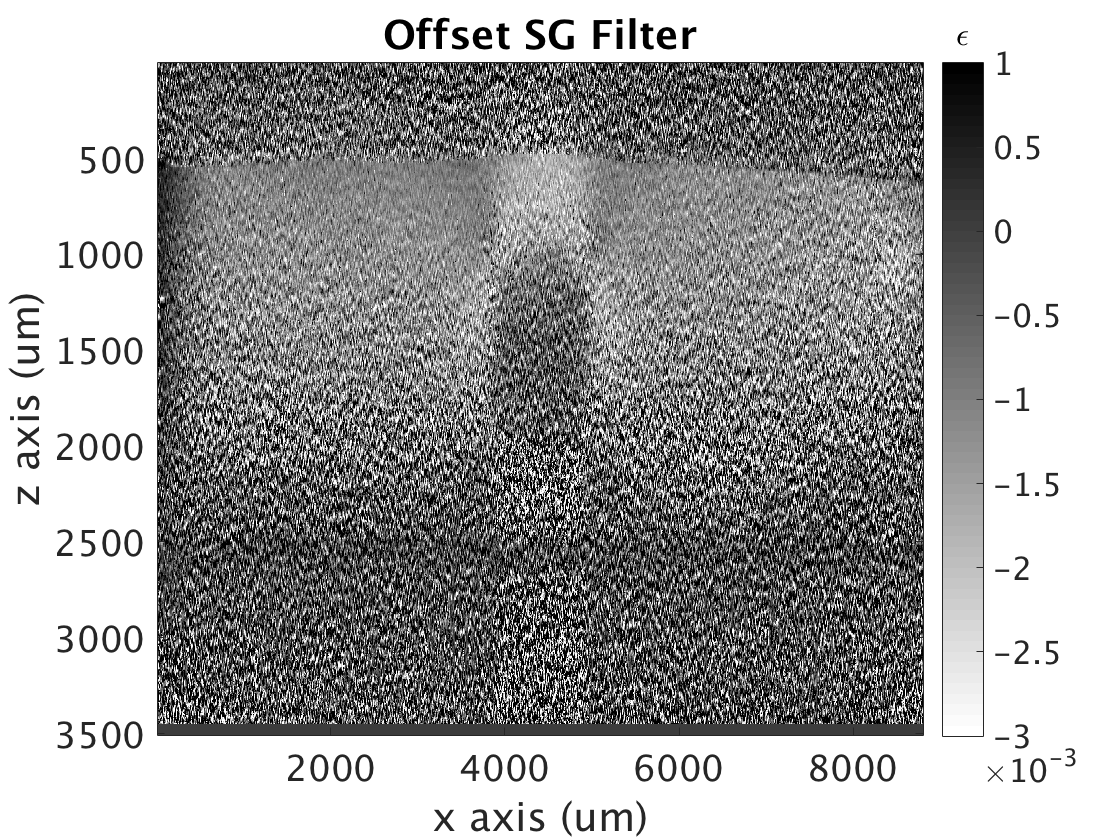
\includegraphics[width=\textwidth]{appendix_figs/posg_fr40_lr0.png}
    \end{subfigure}
    \begin{subfigure}{0.49\textwidth}
    	\centering
        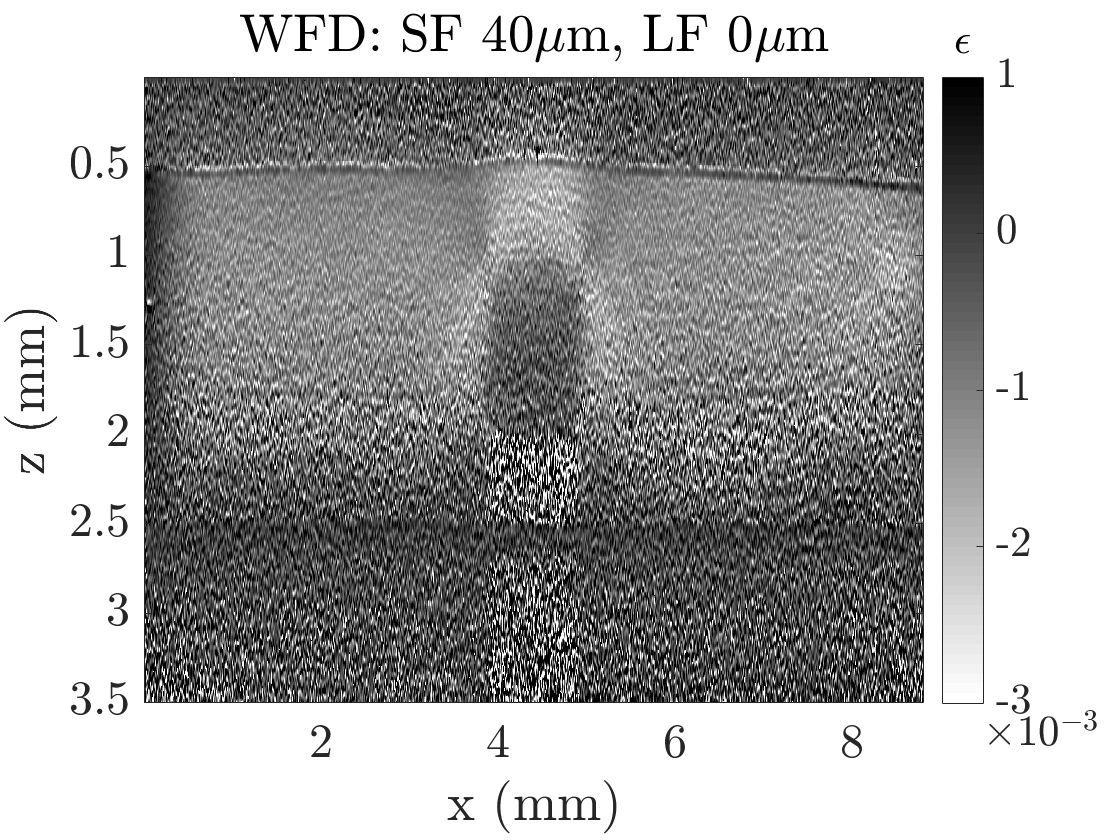
\includegraphics[width=\textwidth]{appendix_figs/wfd_fr40_lr0.png}
    \end{subfigure}
    \\
    \begin{subfigure}{0.49\textwidth}
    	\centering
        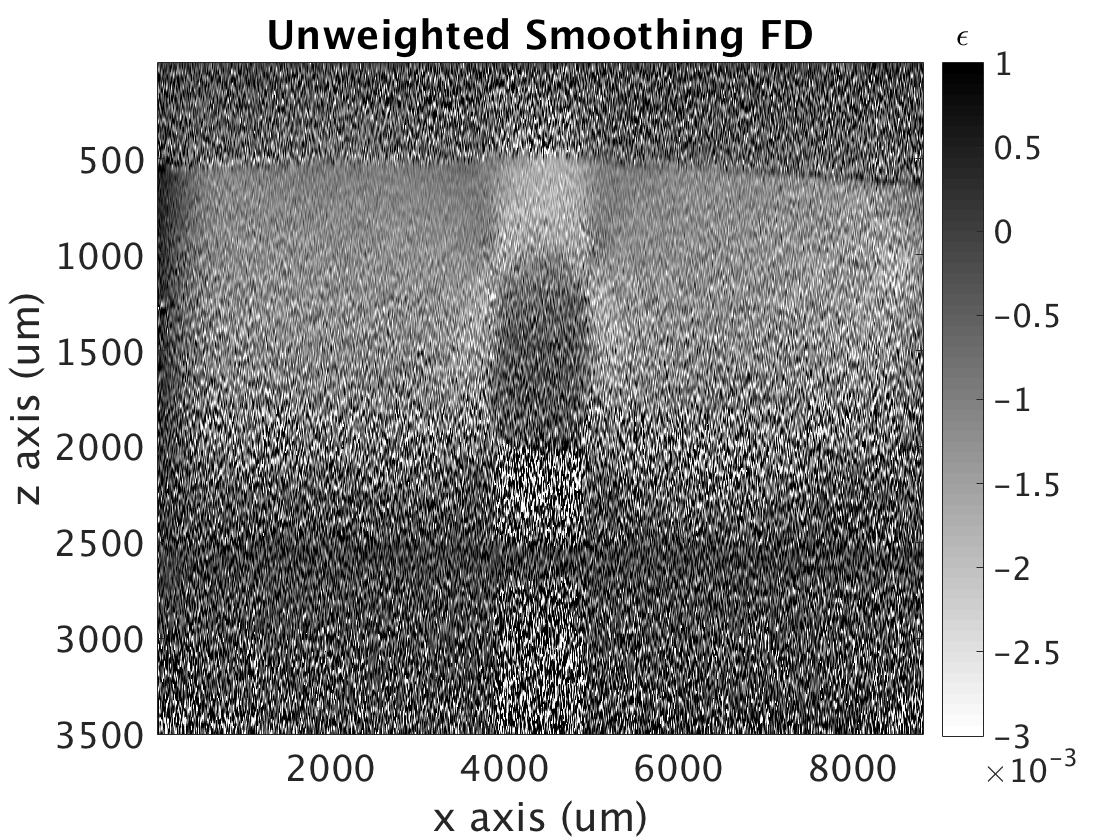
\includegraphics[width=\textwidth]{appendix_figs/uwfd_fr40_lr0.png}
    \end{subfigure}
    \begin{subfigure}{0.49\textwidth}
    	\centering
        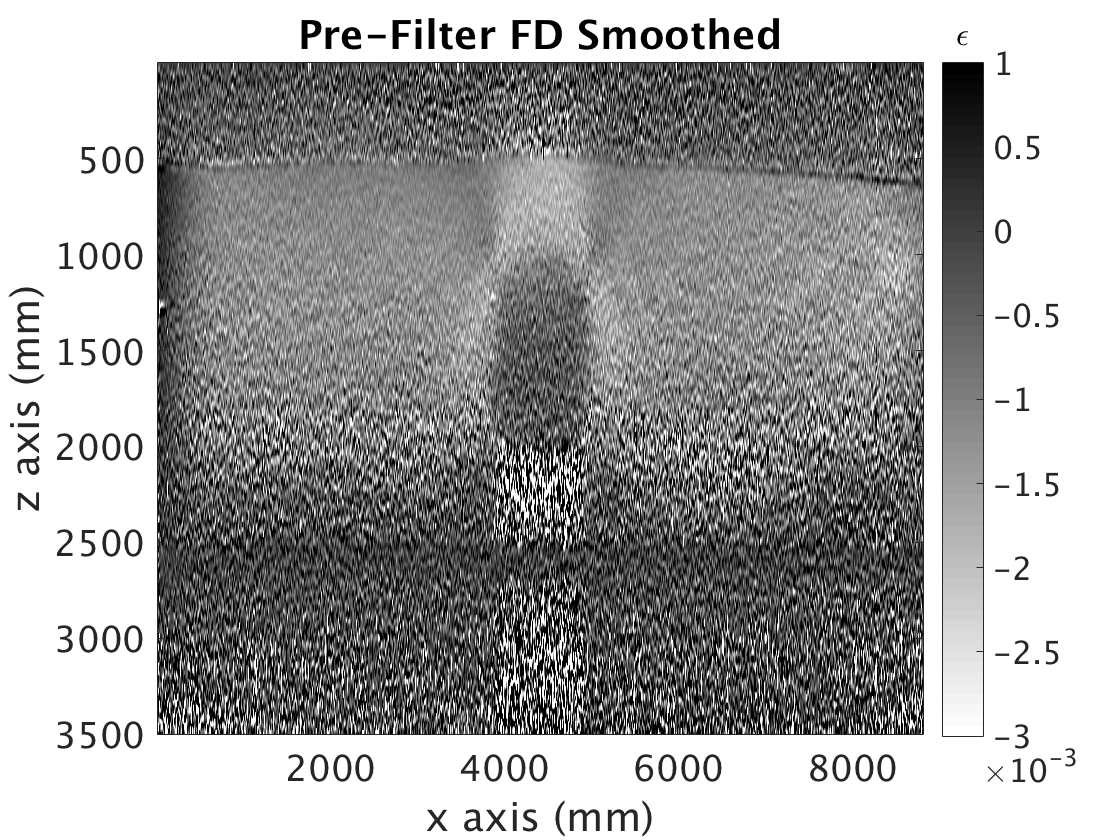
\includegraphics[width=\textwidth]{appendix_figs/fdsm_fr40_lr0.png}
    \end{subfigure}    
    \label{images_low_fitres}
    \caption{Strain B-scans for the different strain estimation techniques, taken at a lower fit resolution of $40\mu m$, with no lateral smoothing.}
\end{figure}

\begin{figure}[h]
	\centering
    \begin{subfigure}{0.49\textwidth}
    	\centering
	    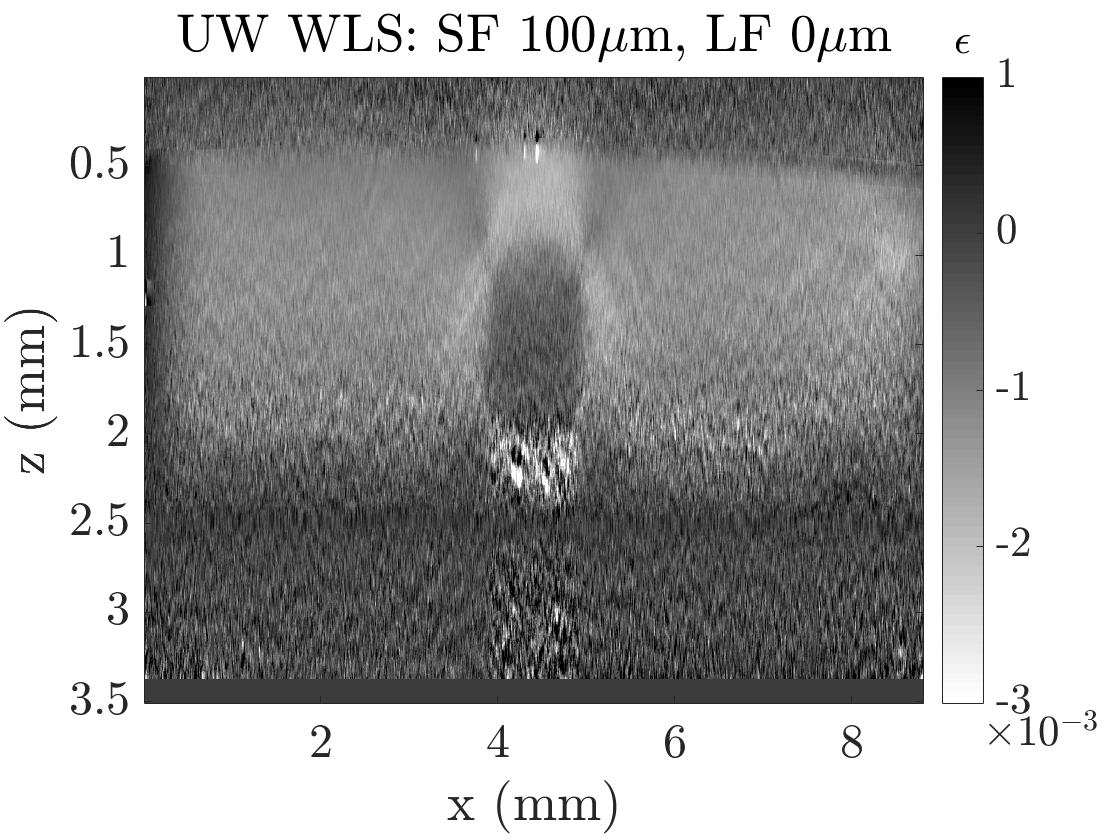
\includegraphics[width=\textwidth]{appendix_figs/wls_fr100_lr0.png}
    \end{subfigure}
    \begin{subfigure}{0.49\textwidth}
    	\centering
        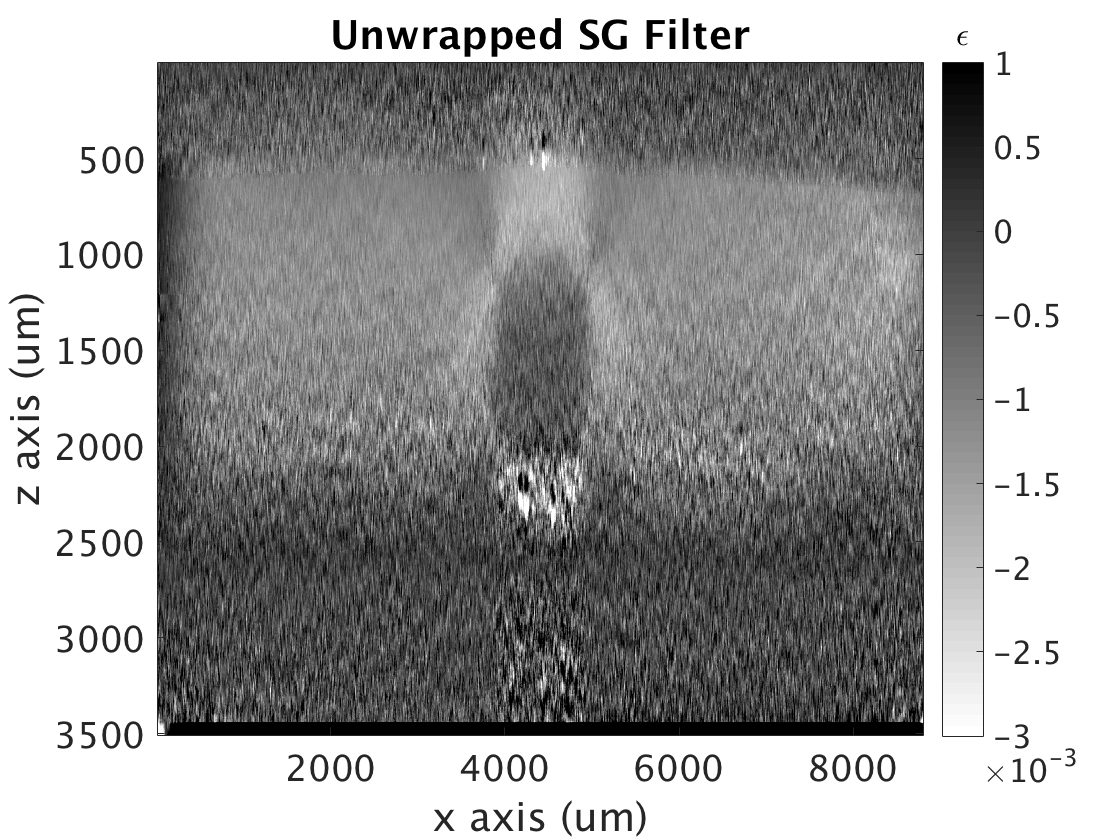
\includegraphics[width=\textwidth]{appendix_figs/uwsg_fr100_lr0.png}
    \end{subfigure}
    \\
    \begin{subfigure}{0.49\textwidth}
    	\centering
        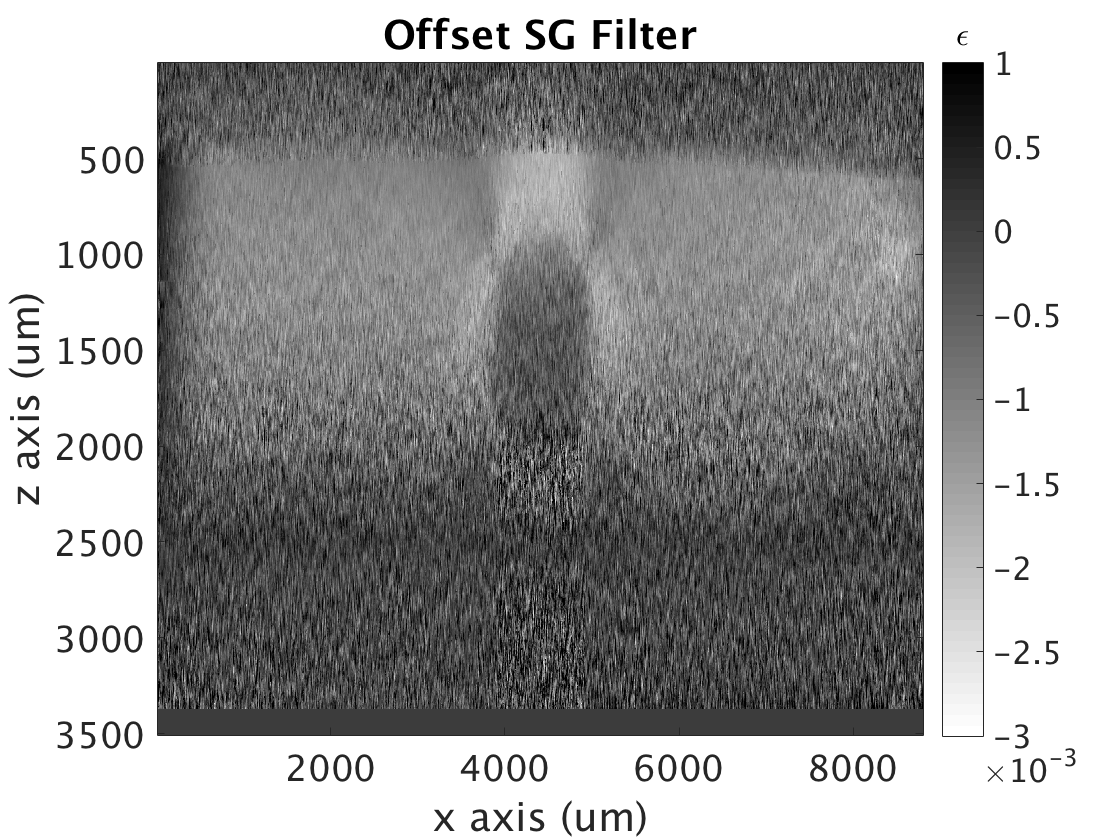
\includegraphics[width=\textwidth]{appendix_figs/posg_fr100_lr0.png}
    \end{subfigure}
    \begin{subfigure}{0.49\textwidth}
    	\centering
        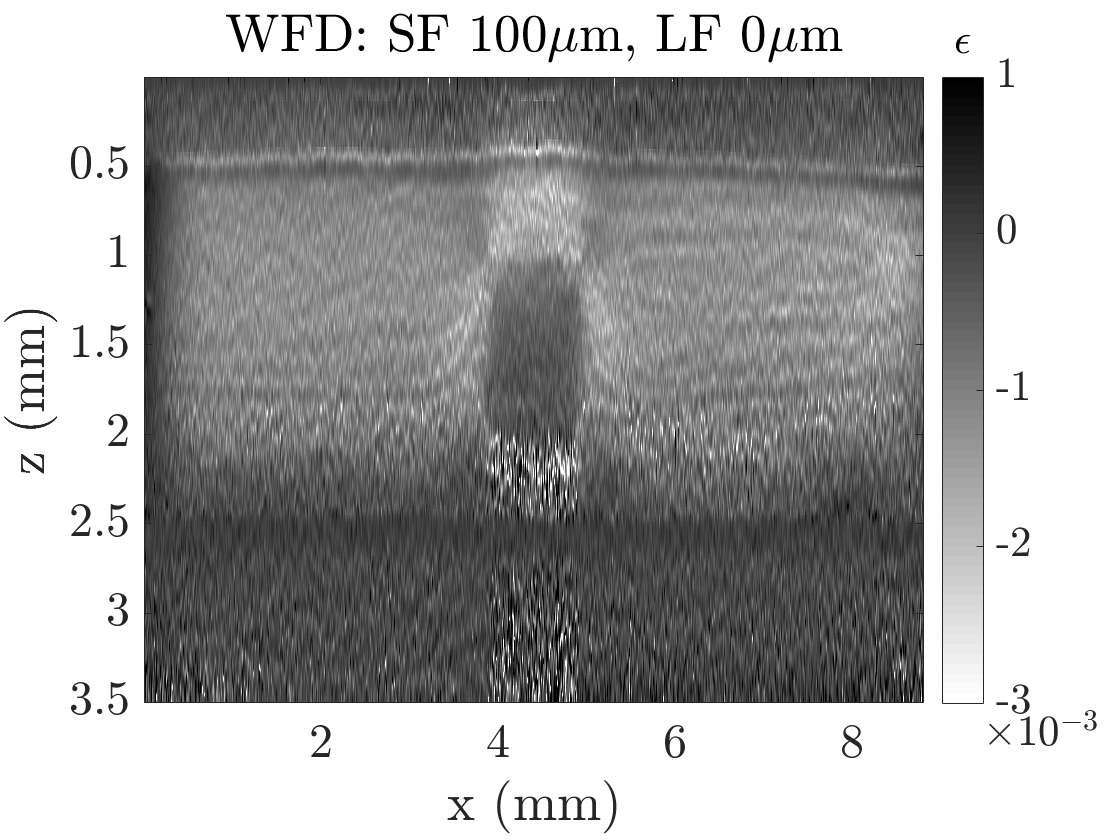
\includegraphics[width=\textwidth]{appendix_figs/wfd_fr100_lr0.png}
    \end{subfigure}
    \\
    \begin{subfigure}{0.49\textwidth}
    	\centering
        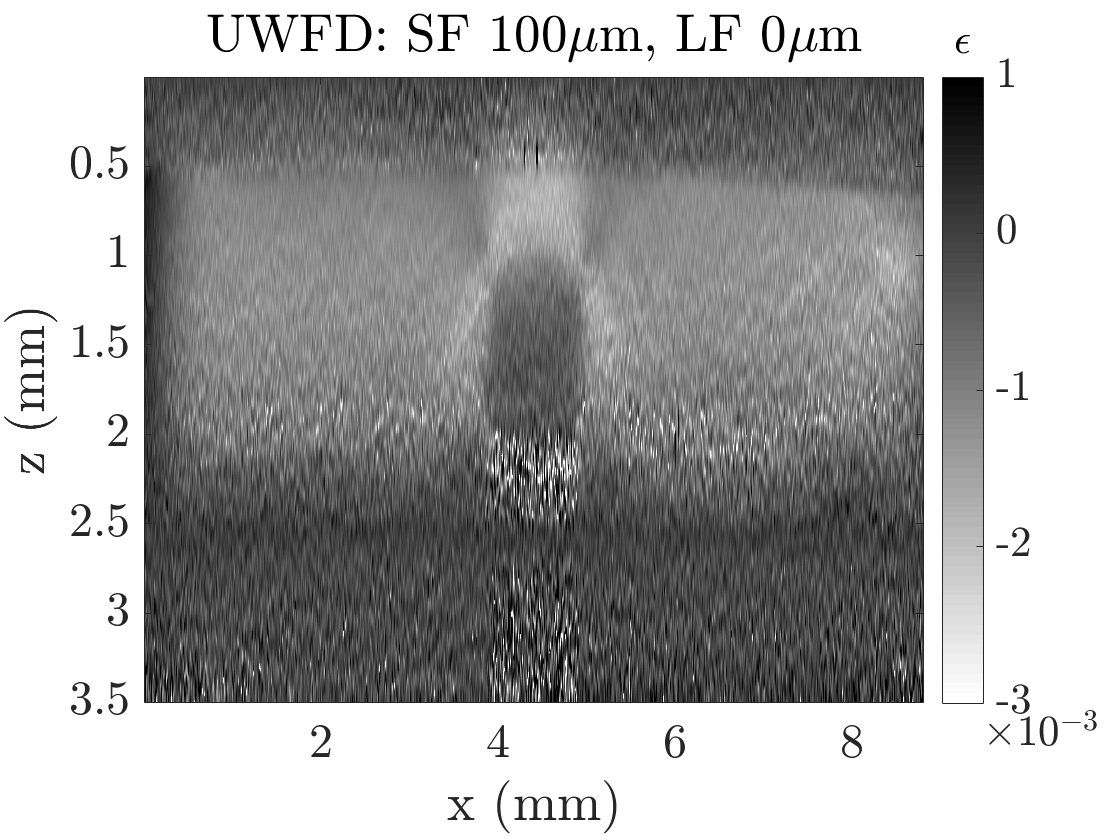
\includegraphics[width=\textwidth]{appendix_figs/uwfd_fr100_lr0.png}
    \end{subfigure}
    \begin{subfigure}{0.49\textwidth}
    	\centering
        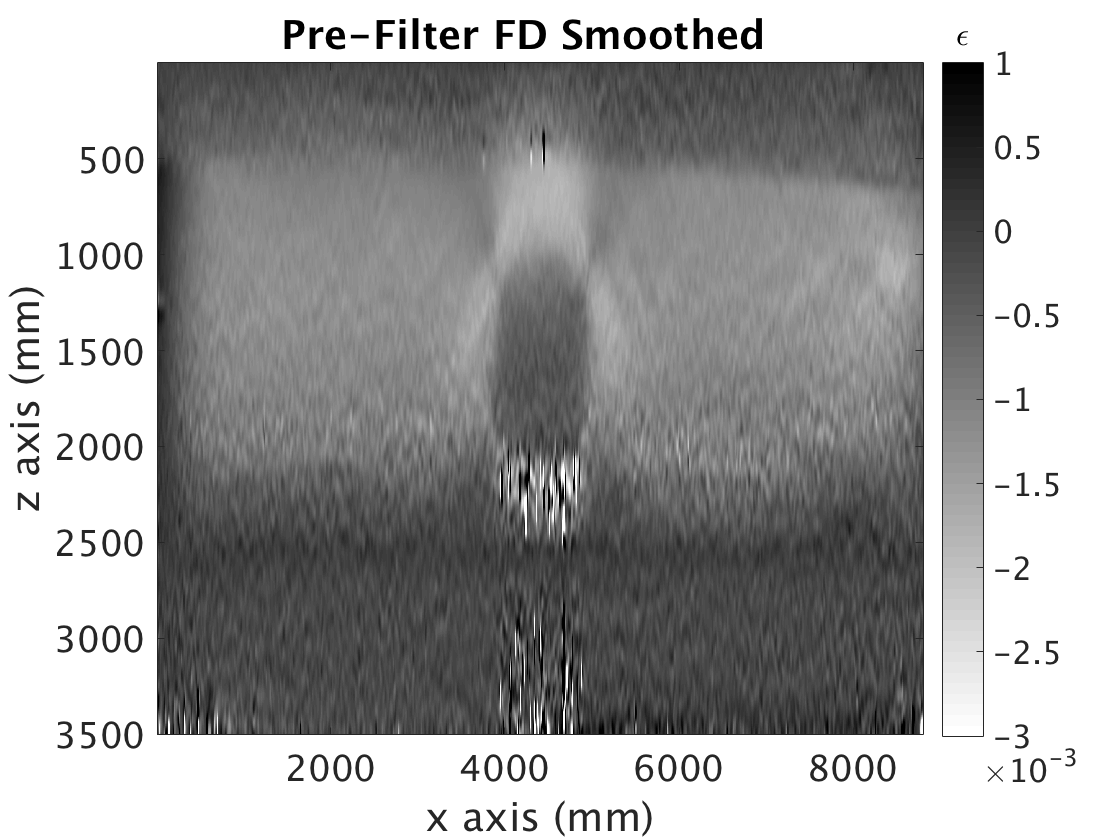
\includegraphics[width=\textwidth]{appendix_figs/fdsm_fr100_lr0.png}
    \end{subfigure}    
    \label{images_high_fitres}
    \caption{Strain B-scans for the different strain estimation techniques, taken at a higher than average fit resolution of $100\mu m$, with no lateral smoothing.}
\end{figure}

%\begin{figure}[h]
%	\centering
%    \begin{subfigure}{0.49\textwidth}
%    	\centering
%        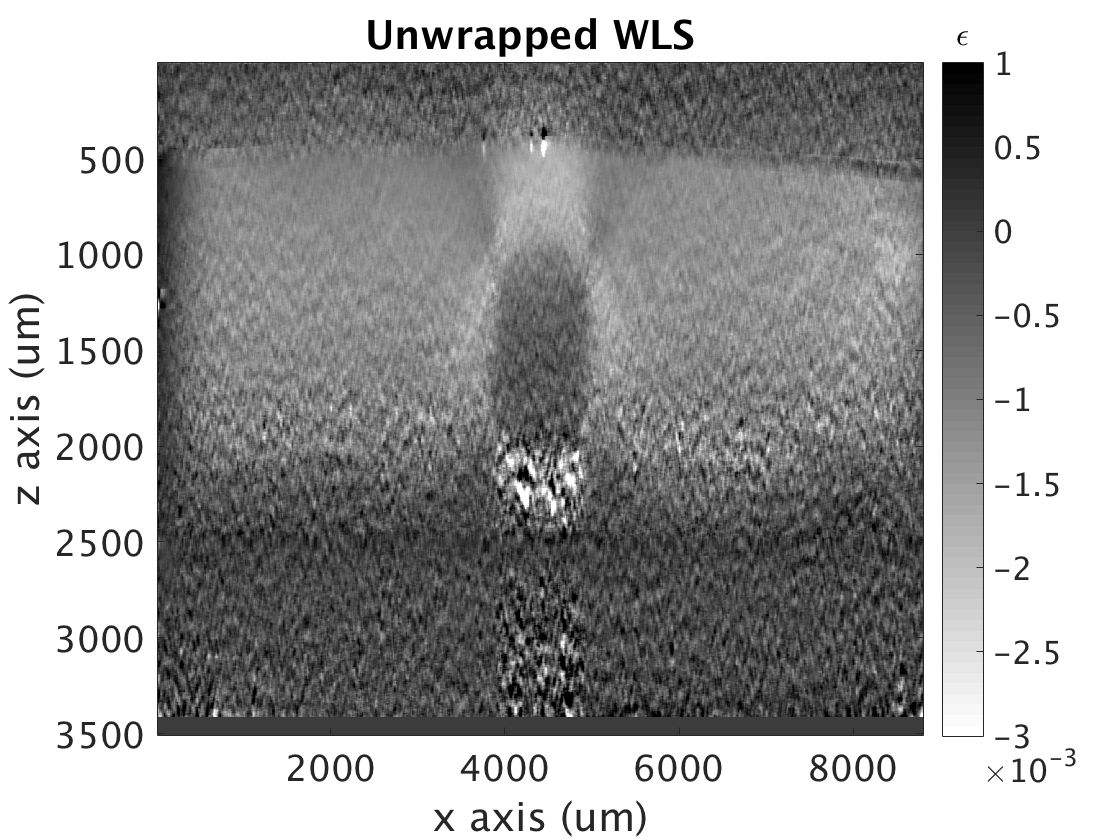
\includegraphics[width=\textwidth]{appendix_figs/wls_fr70_lr20.png}
%    \end{subfigure}
%    \begin{subfigure}{0.49\textwidth}
%    	\centering
%        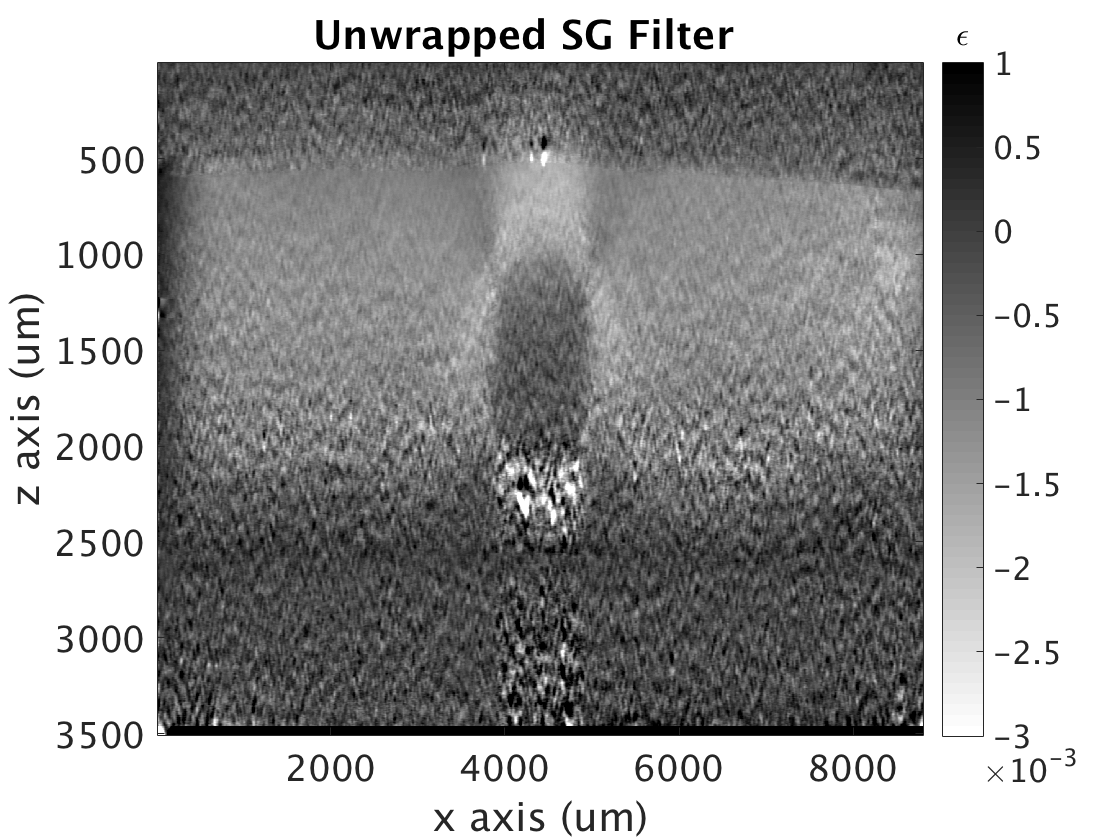
\includegraphics[width=\textwidth]{appendix_figs/uwsg_fr70_lr20.png}
%    \end{subfigure}
%    \\
%    \begin{subfigure}{0.49\textwidth}
%    	\centering
%        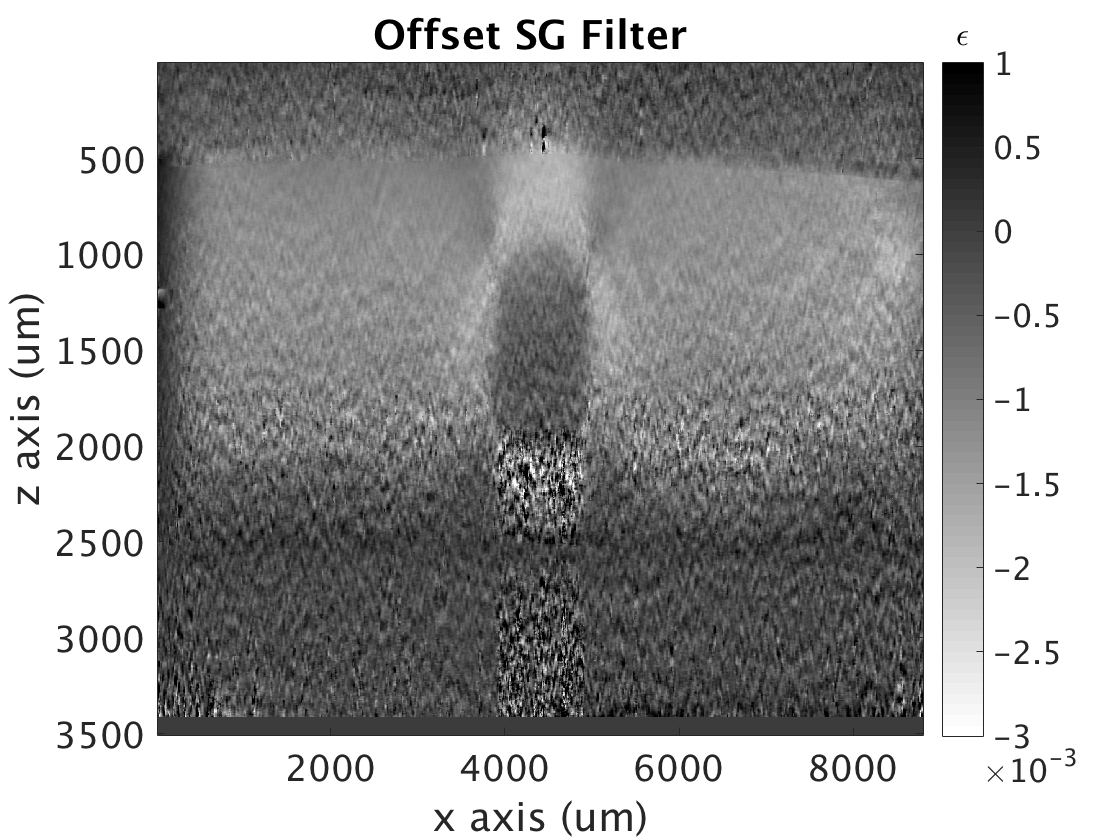
\includegraphics[width=\textwidth]{appendix_figs/posg_fr70_lr20.png}
%    \end{subfigure}
%    \begin{subfigure}{0.49\textwidth}
%    	\centering
%        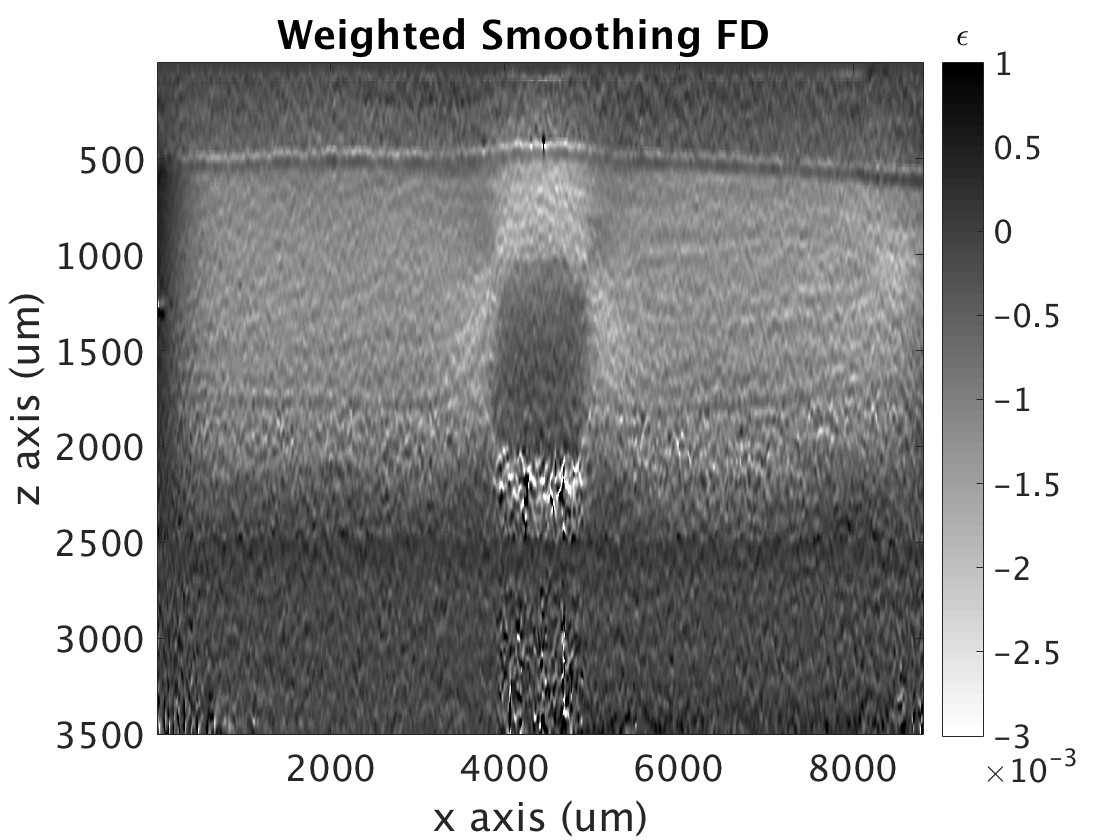
\includegraphics[width=\textwidth]{appendix_figs/wfd_fr70_lr20.png}
%    \end{subfigure}
%    \\
%    \begin{subfigure}{0.49\textwidth}
%    	\centering
%        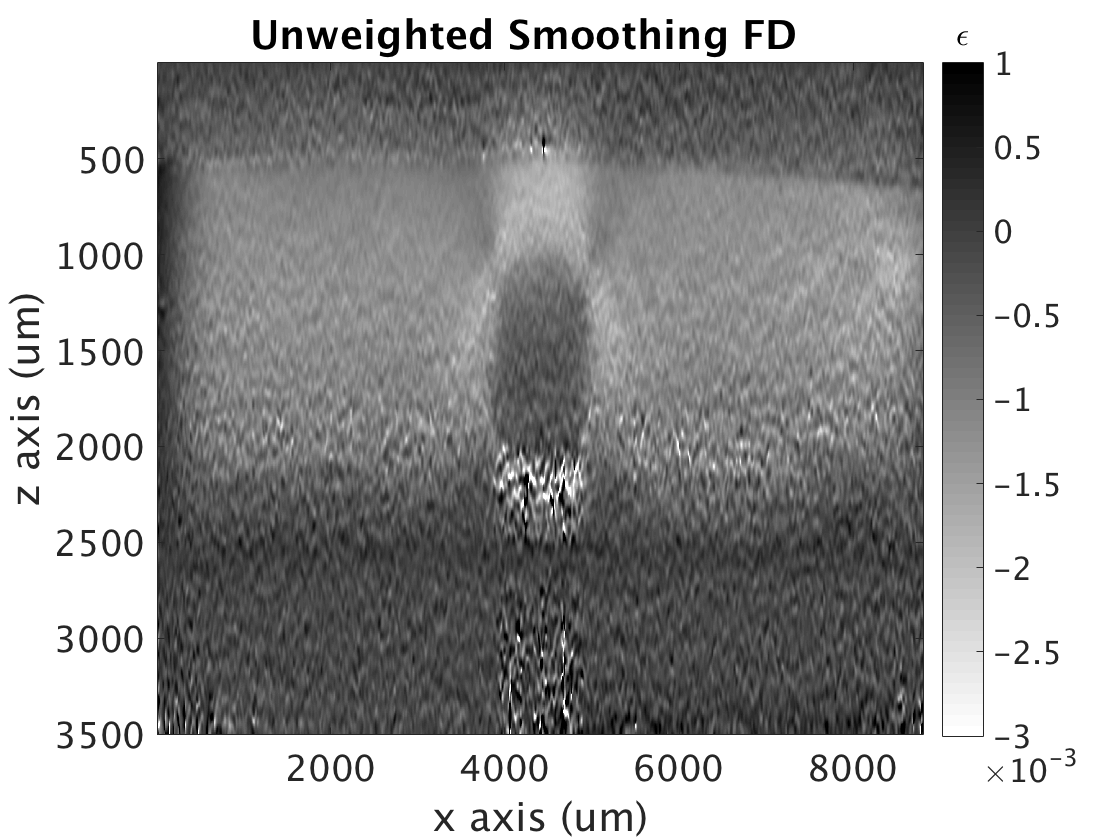
\includegraphics[width=\textwidth]{appendix_figs/uwfd_fr70_lr20.png}
%    \end{subfigure}
%    \begin{subfigure}{0.49\textwidth}
%    	\centering
%        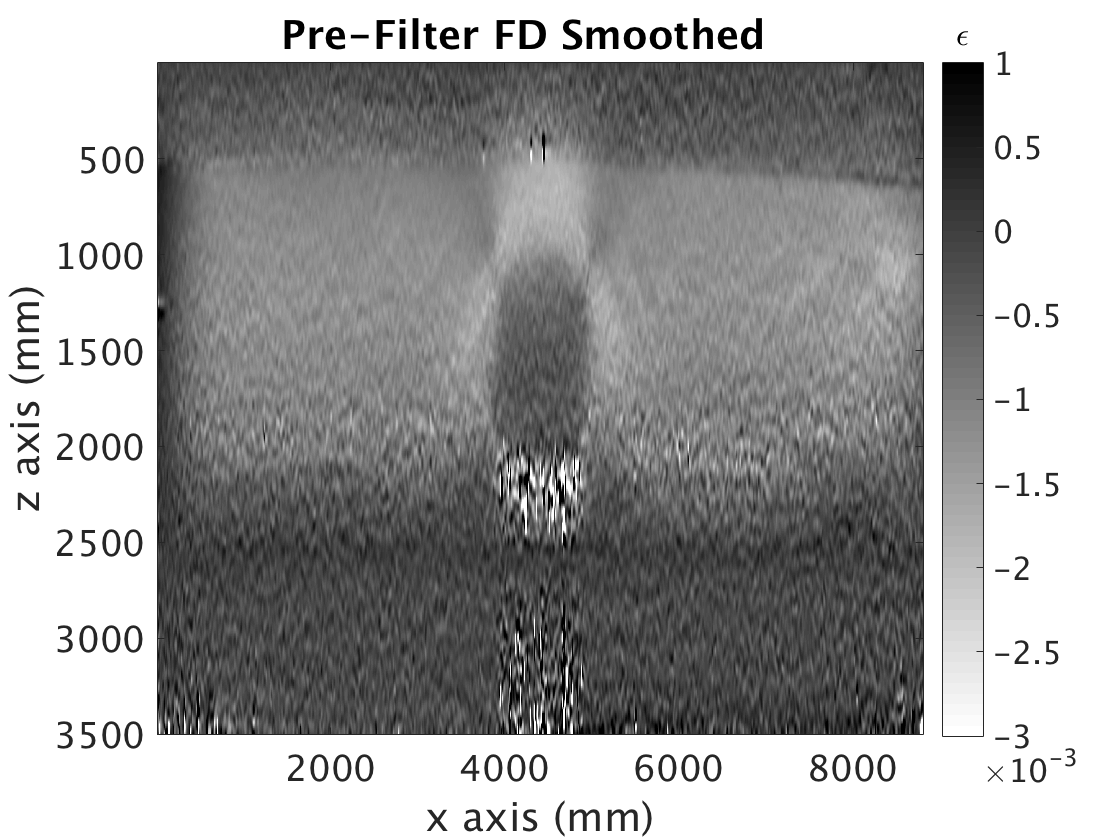
\includegraphics[width=\textwidth]{appendix_figs/fdsm_fr70_lr20.png}
%    \end{subfigure}    
%    \label{images_low_fitres}
%    \caption{Strain B-scans for the different strain estimation techniques, at the standard fit resolution ($70 \mu m$ but with added lateral smoothing of resolution $20 \mu m$.}
%\end{figure}

\begin{figure}[h]
	\centering
    \begin{subfigure}{0.49\textwidth}
    	\centering
        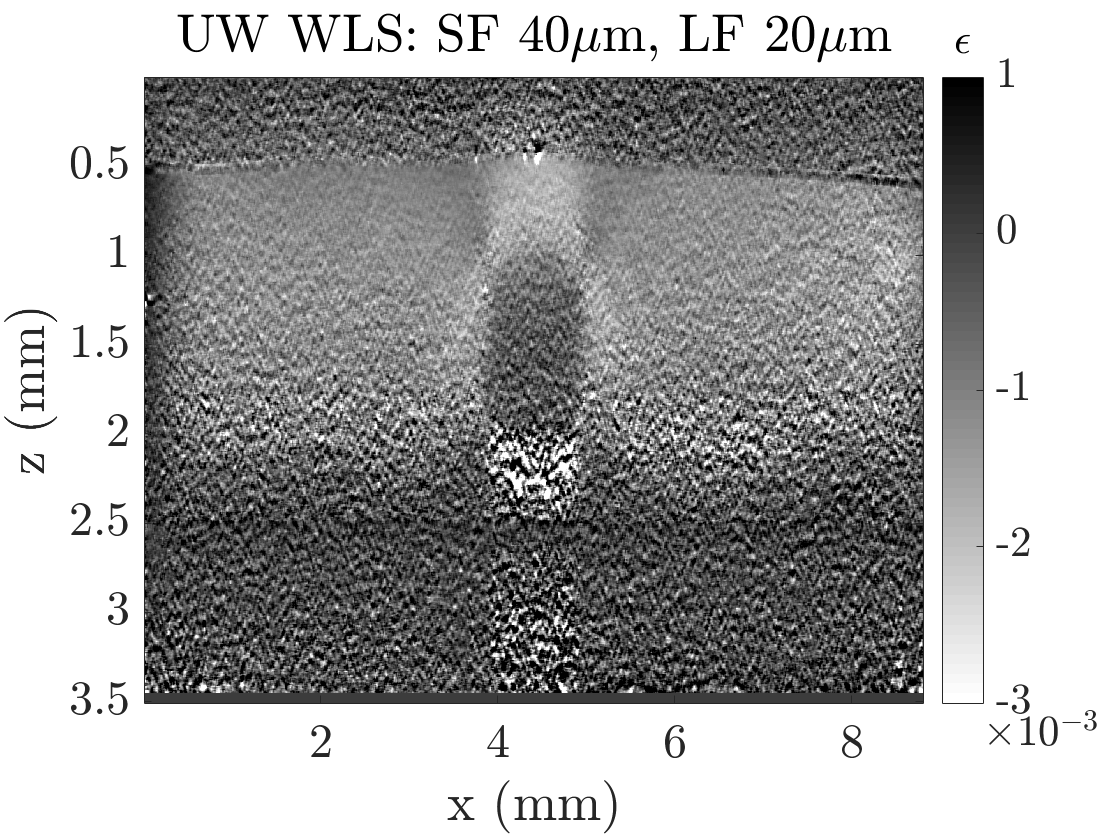
\includegraphics[width=\textwidth]{appendix_figs/wls_fr40_lr20.png}
    \end{subfigure}
    \begin{subfigure}{0.49\textwidth}
    	\centering
        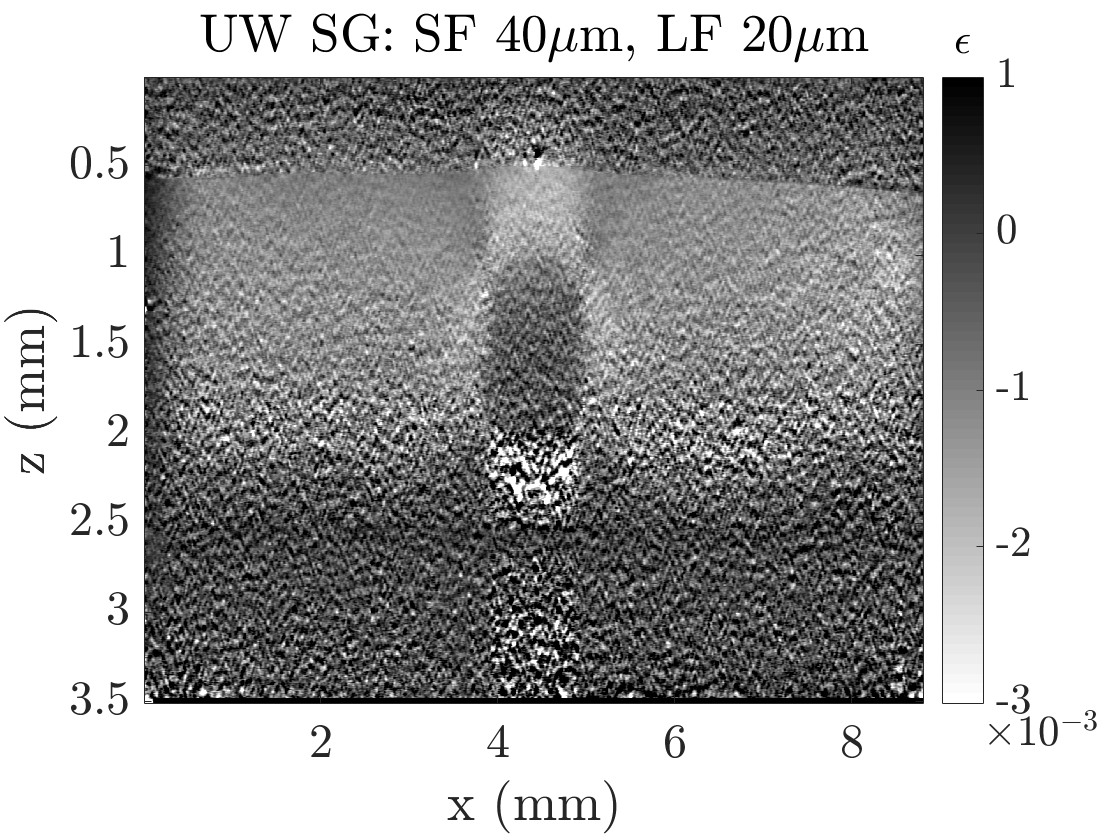
\includegraphics[width=\textwidth]{appendix_figs/uwsg_fr40_lr20.png}
    \end{subfigure}
    \\
    \begin{subfigure}{0.49\textwidth}
    	\centering
        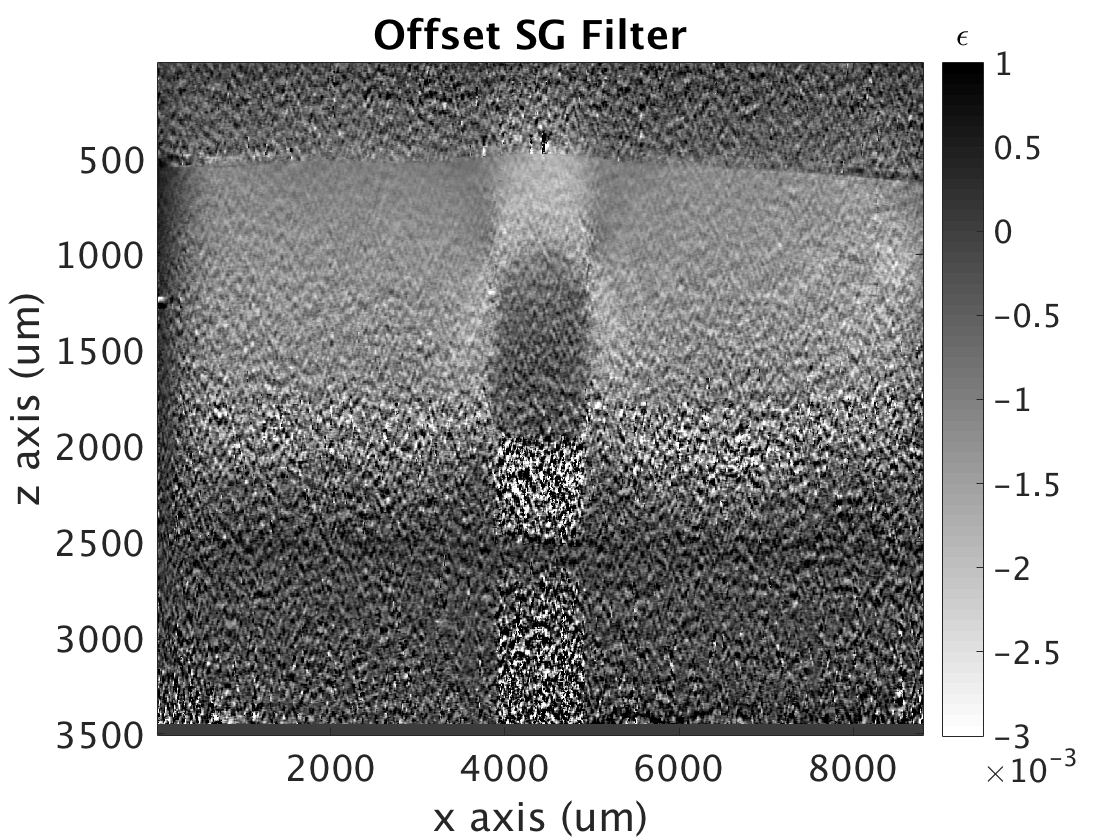
\includegraphics[width=\textwidth]{appendix_figs/posg_fr40_lr20.png}
    \end{subfigure}
    \begin{subfigure}{0.49\textwidth}
    	\centering
        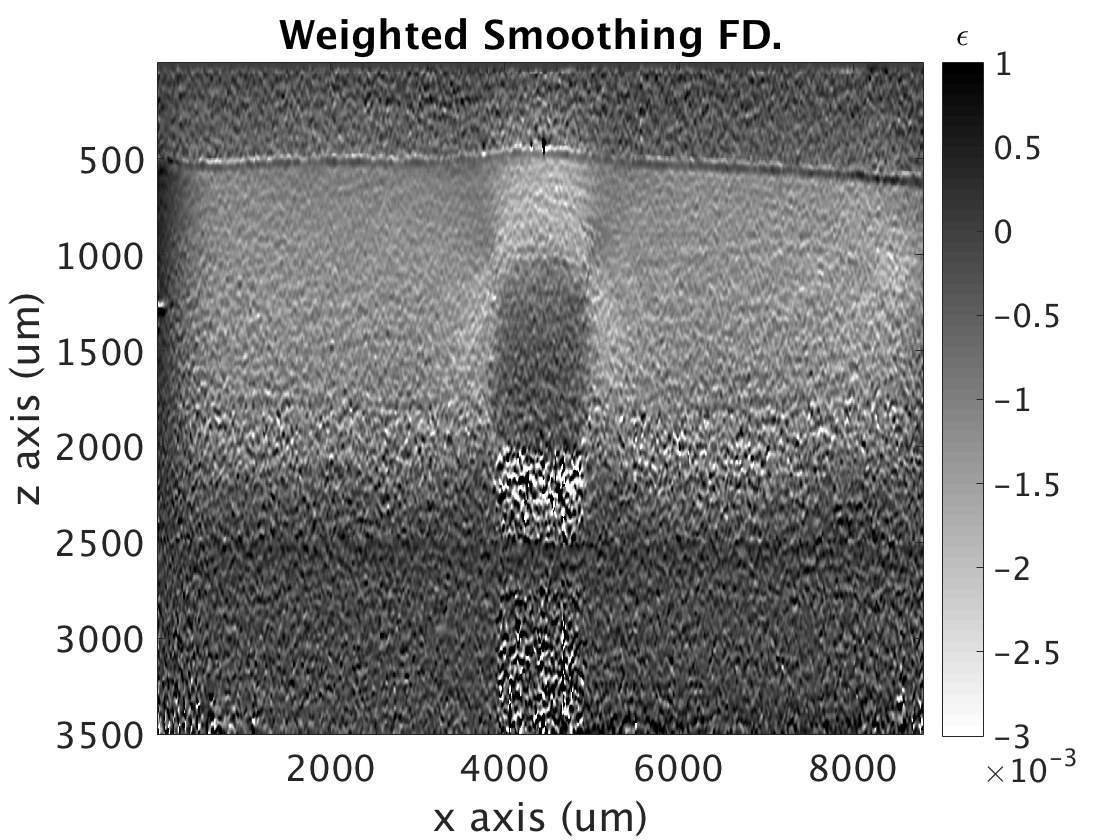
\includegraphics[width=\textwidth]{appendix_figs/wfd_fr40_lr20.png}
    \end{subfigure}
    \\
    \begin{subfigure}{0.49\textwidth}
    	\centering
        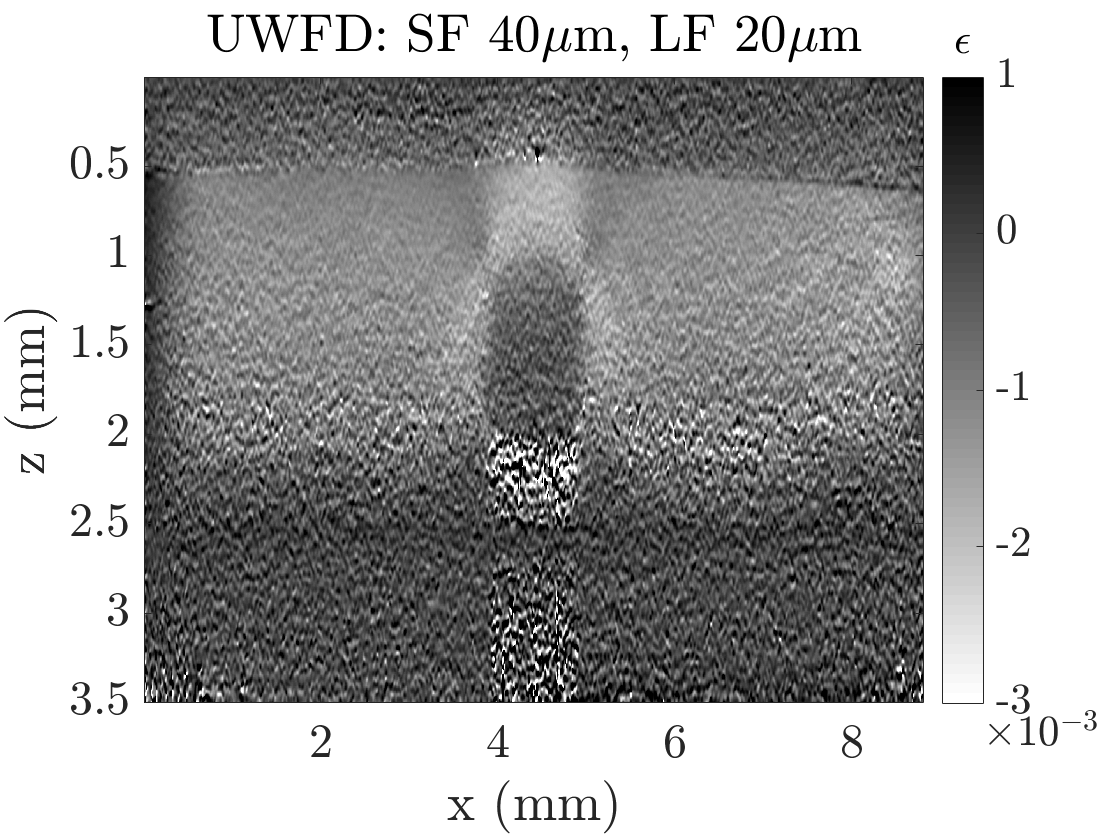
\includegraphics[width=\textwidth]{appendix_figs/uwfd_fr40_lr20.png}
    \end{subfigure}
    \begin{subfigure}{0.49\textwidth}
    	\centering
        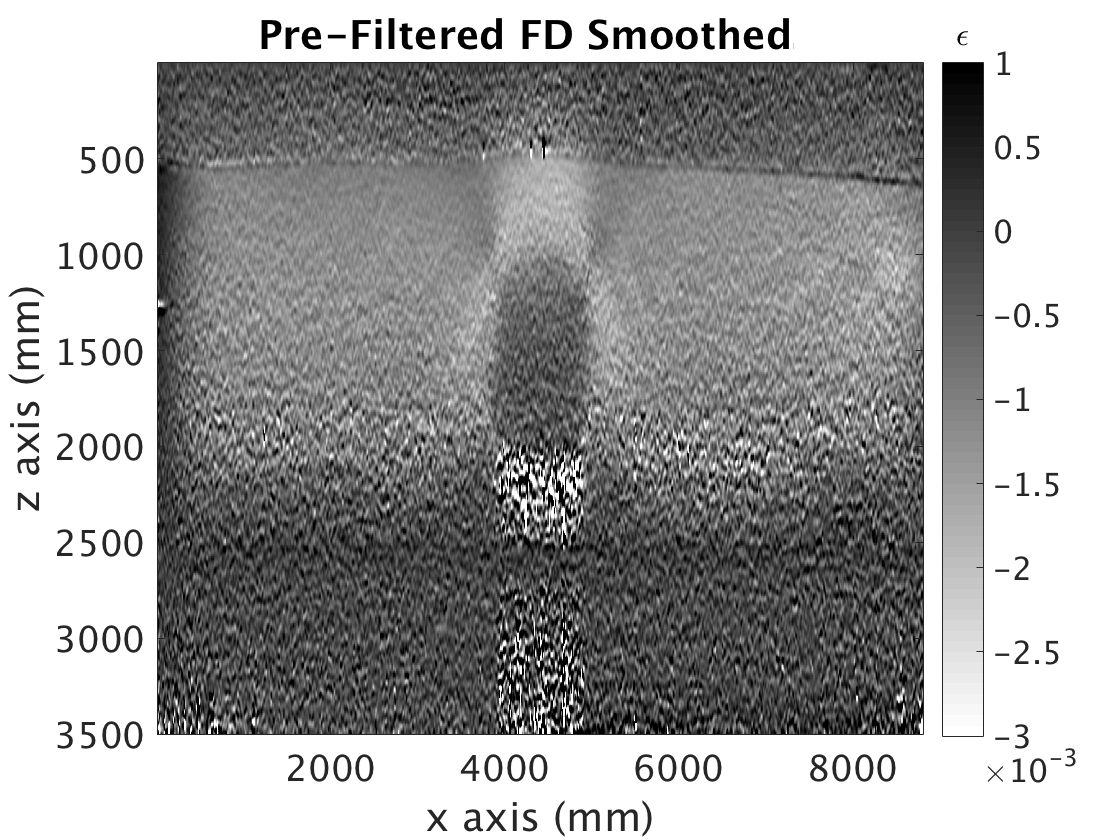
\includegraphics[width=\textwidth]{appendix_figs/fdsm_fr40_lr20.png}
    \end{subfigure}    
    \label{images_low_fitres}
    \caption{Strain B-scans for the different strain estimation techniques, taken at a lower fit resolution of $40\mu m$, with lateral smoothing of $20 \mu m$ resolution.}
\end{figure}

%\begin{figure}[h]
%	\centering
%    \begin{subfigure}{0.49\textwidth}
%    	\centering
%        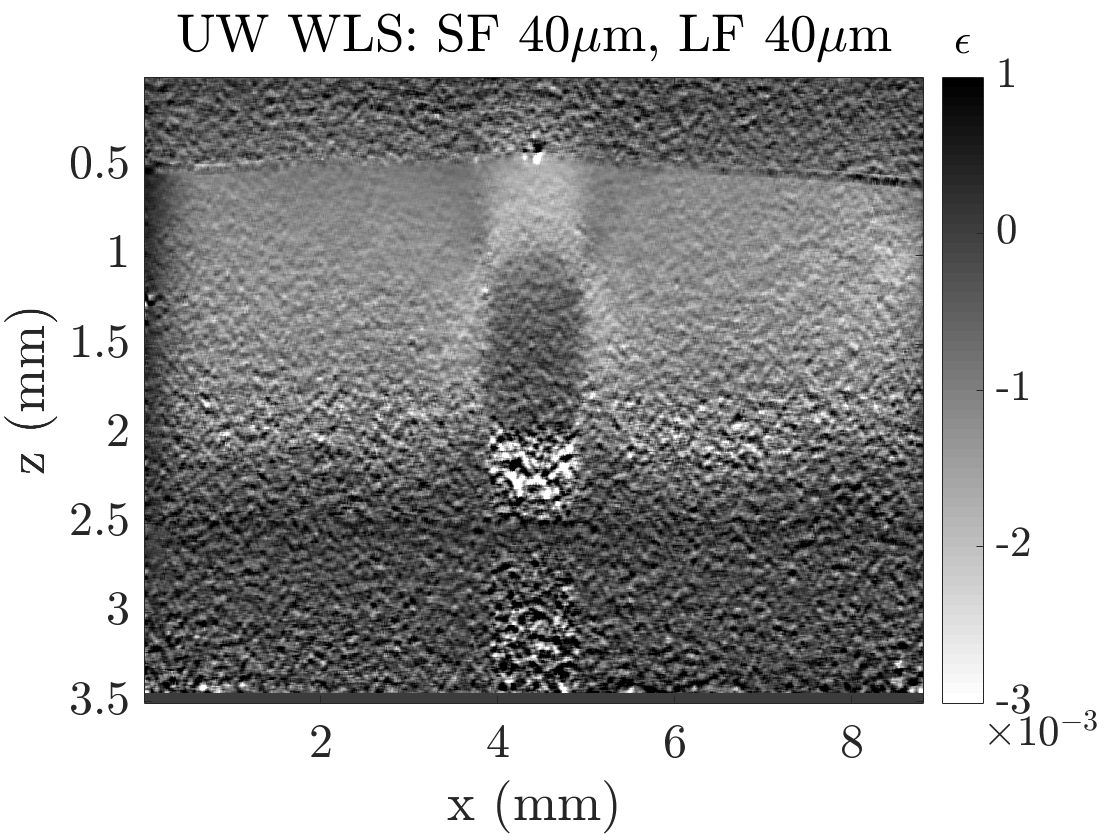
\includegraphics[width=\textwidth]{appendix_figs/wls_fr40_lr40.png}
%    \end{subfigure}
%    \begin{subfigure}{0.49\textwidth}
%    	\centering
%        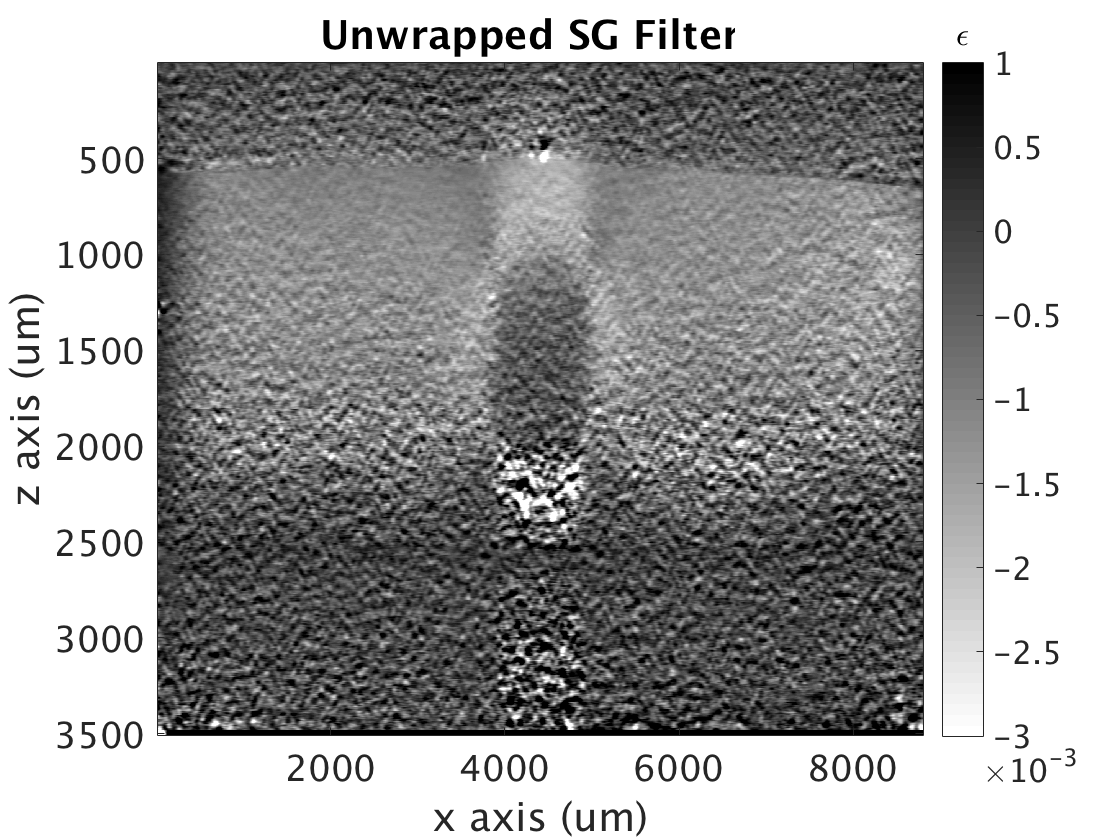
\includegraphics[width=\textwidth]{appendix_figs/uwsg_fr40_lr40.png}
%    \end{subfigure}
%    \\
%    \begin{subfigure}{0.49\textwidth}
%    	\centering
%        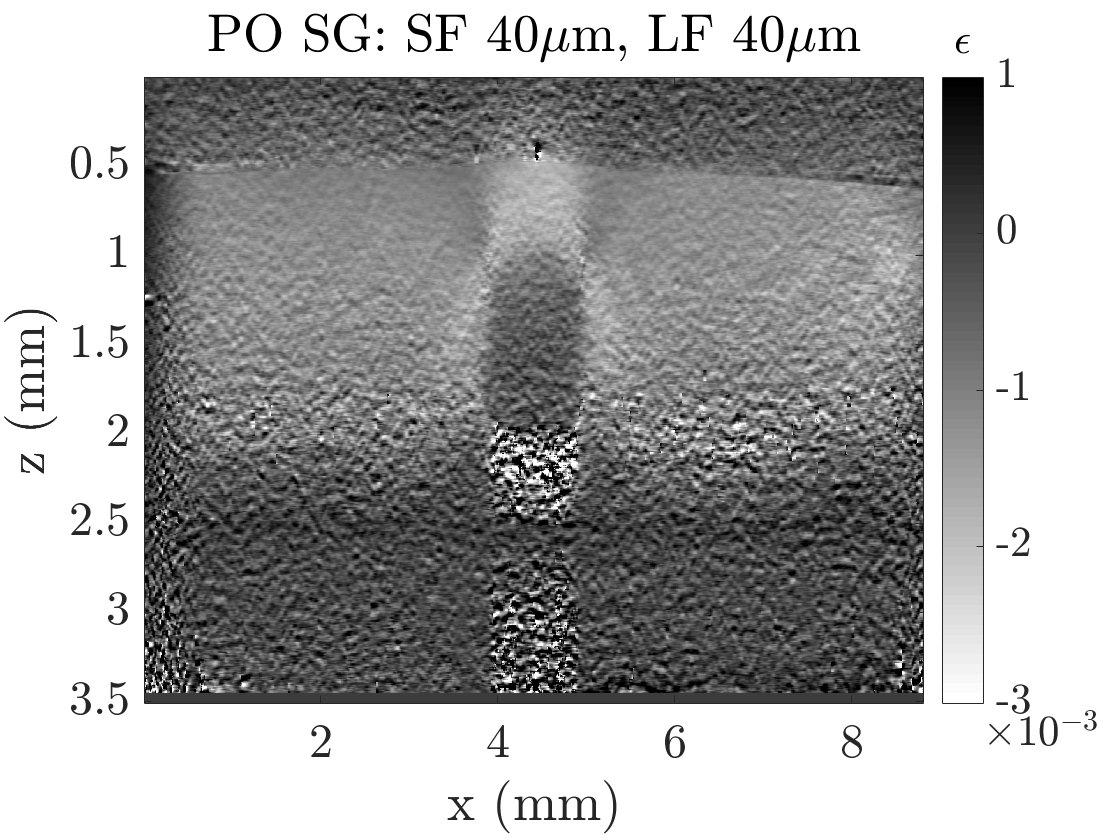
\includegraphics[width=\textwidth]{appendix_figs/posg_fr40_lr40.png}
%    \end{subfigure}
%    \begin{subfigure}{0.49\textwidth}
%    	\centering
%        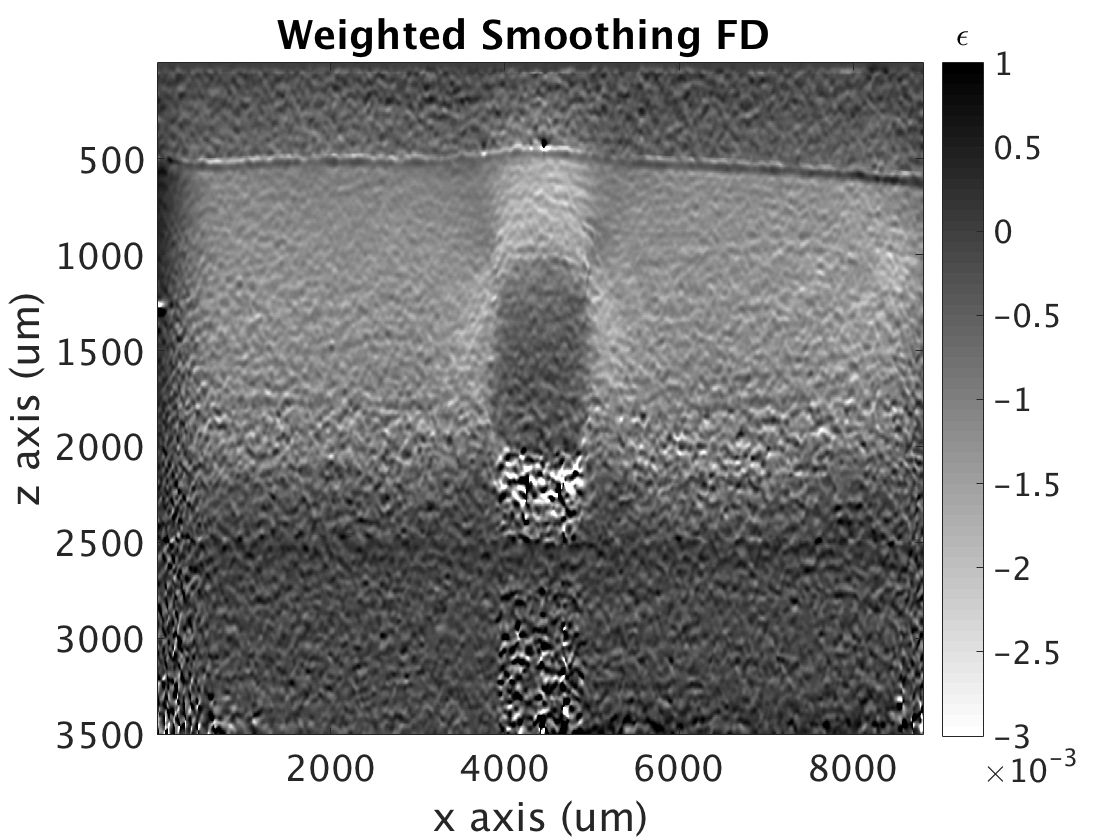
\includegraphics[width=\textwidth]{appendix_figs/wfd_fr40_lr40.png}
%    \end{subfigure}
%    \\
%    \begin{subfigure}{0.49\textwidth}
%    	\centering
%        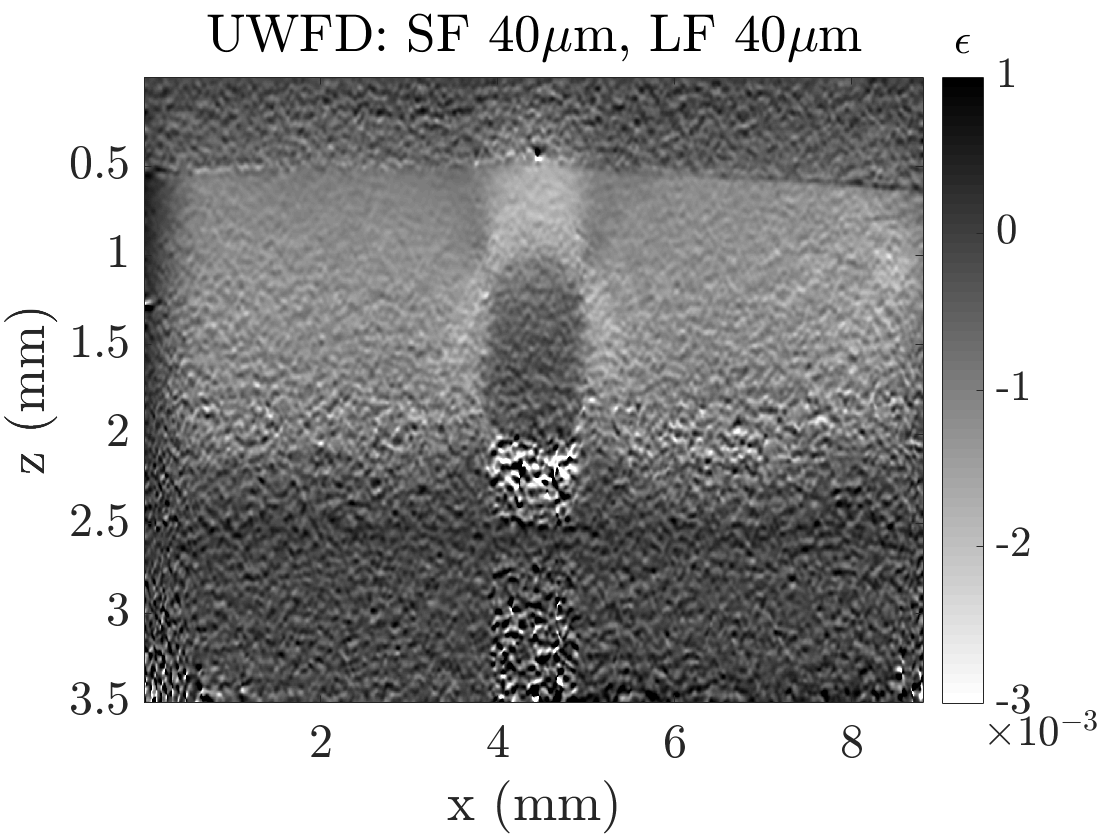
\includegraphics[width=\textwidth]{appendix_figs/uwfd_fr40_lr40.png}
%    \end{subfigure}
%    \begin{subfigure}{0.49\textwidth}
%    	\centering
%        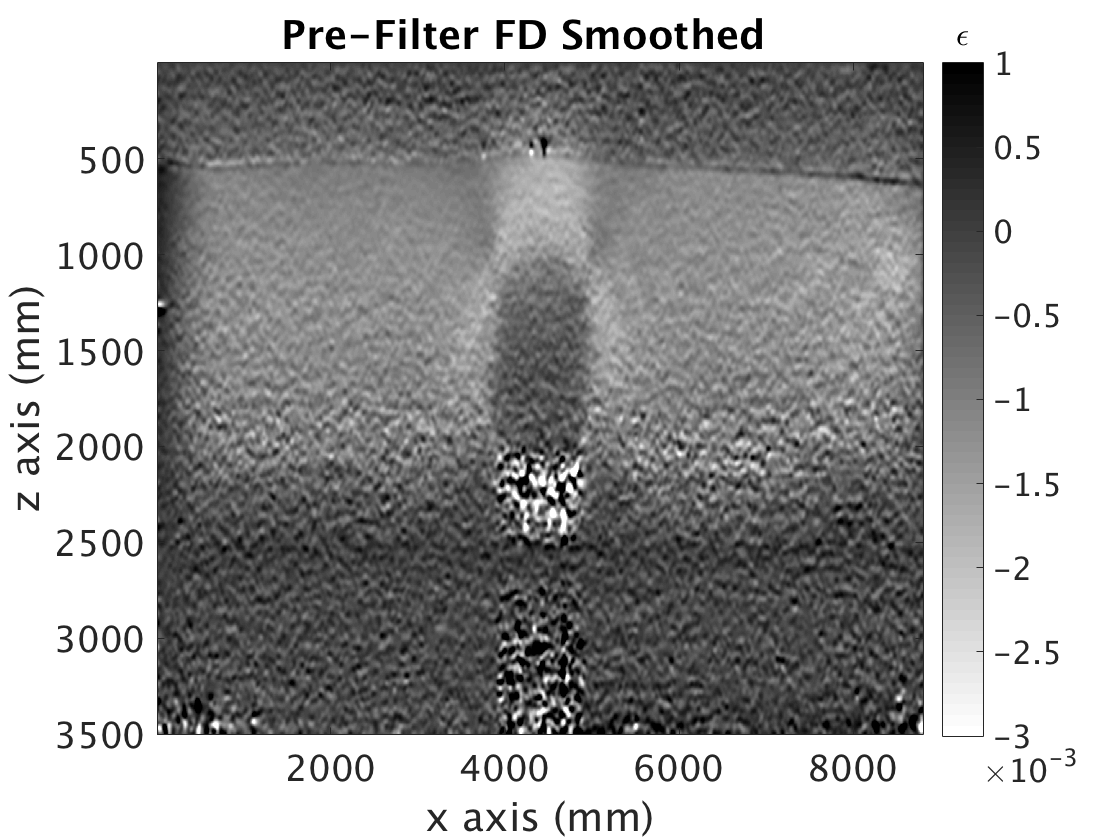
\includegraphics[width=\textwidth]{appendix_figs/fdsm_fr40_lr40.png}
%    \end{subfigure}    
%    \label{images_low_fitres}
%    \caption{Strain B-scans for the different strain estimation techniques, taken at a lower fit resolution of $40\mu m$, with a higher lateral smoothing of $40 \mu m$ resolution.}
%\end{figure}

